% -*- mode: latex; mode: flyspell; ispell-local-dictionary: "en_US"; coding: utf-8; fill-column: 80 -*-

\documentclass{article}

\usepackage[utf8]{inputenc}
\usepackage[english]{babel}

\usepackage{amsmath,amsfonts,amssymb}
\usepackage{fullpage}
\usepackage{verbatim}

\usepackage{tikz,pgfplots}

\pgfplotsset{
  width=150mm,height=100mm,
  major grid style={thin,dotted,color=black!50},
  minor grid style={thin,dotted,color=black!50},
  grid,
  every axis/.append style={
    line width=0.5pt,
    tick style={
      line cap=round,
      thin,
      major tick length=4pt,
      minor tick length=2pt,
    },
  },
  legend cell align=left,
  legend pos=north west,
}

%%%%%%%%%%%%%%%%%%%%%%%%%%%%%%%%%%%%%%%%%%%%%%%%%%%%%%%%%%%%%%%%%%%%%%%%%%%%%%%%

\begin{document}

\title{Sorting Speed Example}
\author{Tim Tannert}
\maketitle

% IMPORT-DATA hashmap stats_hashmap_size.txt
% IMPORT-DATA mphf stats_mphf_size.txt


\begin{center}
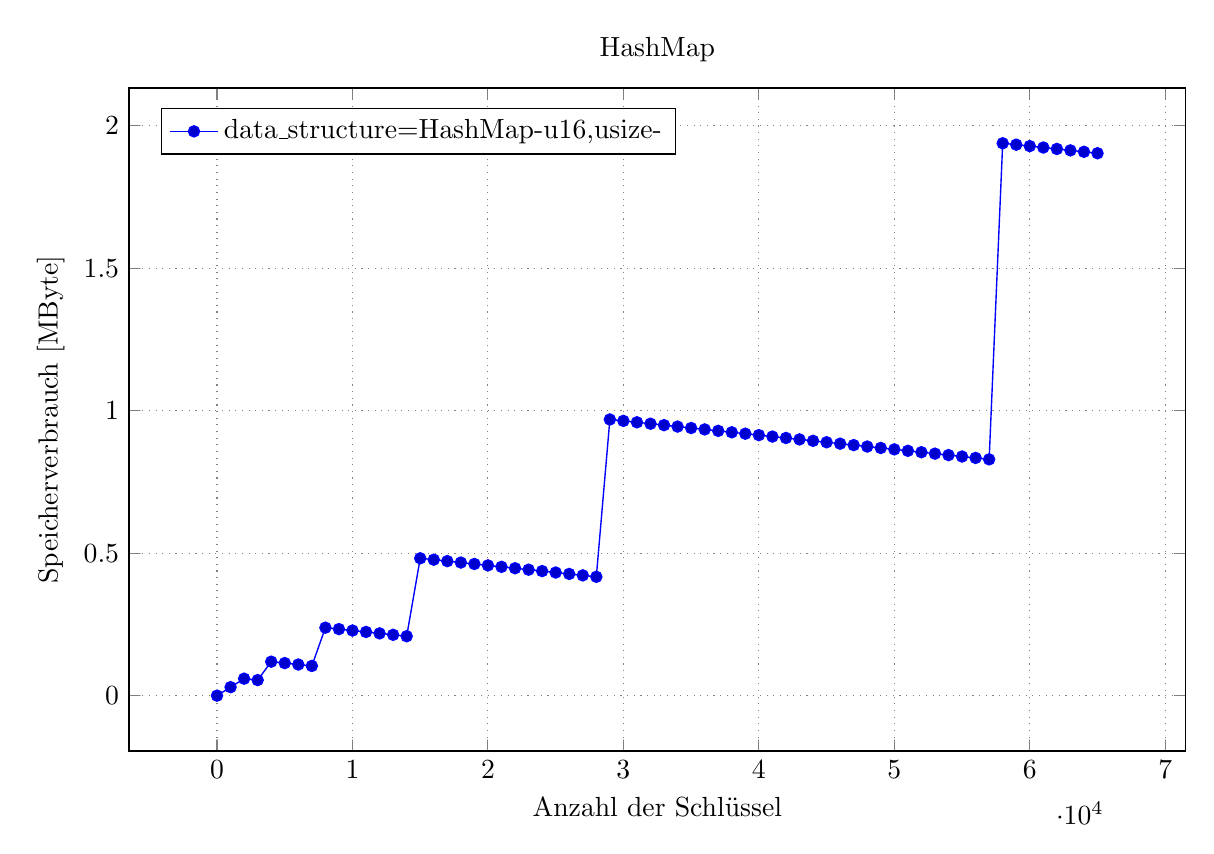
\begin{tikzpicture}
  \begin{axis}[
    title={HashMap},
    xlabel={Anzahl der Schlüssel},
    ylabel={Speicherverbrauch [MByte]},
    ]

    %% MULTIPLOT(data_structure) SELECT size AS x, size_bytes/1e6 AS y, MULTIPLOT
    %% FROM hashmap GROUP BY MULTIPLOT,x ORDER BY MULTIPLOT,x
    \addplot coordinates { (1,0.000107) (1001,0.029883) (2001,0.059699) (3001,0.054699) (4001,0.119331) (5001,0.114331) (6001,0.109331) (7001,0.104331) (8001,0.238595) (9001,0.233595) (10001,0.228595) (11001,0.223595) (12001,0.218595) (13001,0.213595) (14001,0.208595) (15001,0.482123) (16001,0.477123) (17001,0.472123) (18001,0.467123) (19001,0.462123) (20001,0.457123) (21001,0.452123) (22001,0.447123) (23001,0.442123) (24001,0.437123) (25001,0.432123) (26001,0.427123) (27001,0.422123) (28001,0.417123) (29001,0.969179) (30001,0.964179) (31001,0.959179) (32001,0.954179) (33001,0.949179) (34001,0.944179) (35001,0.939179) (36001,0.934179) (37001,0.929179) (38001,0.924179) (39001,0.919179) (40001,0.914179) (41001,0.909179) (42001,0.904179) (43001,0.899179) (44001,0.894179) (45001,0.889179) (46001,0.884179) (47001,0.879179) (48001,0.874179) (49001,0.869179) (50001,0.864179) (51001,0.859179) (52001,0.854179) (53001,0.849179) (54001,0.844179) (55001,0.839179) (56001,0.834179) (57001,0.829179) (58001,1.938291) (59001,1.933291) (60001,1.928291) (61001,1.923291) (62001,1.918291) (63001,1.913291) (64001,1.908291) (65001,1.903291) };
    \addlegendentry{data\_structure=HashMap-u16,usize-};
    
    
  \end{axis}
\end{tikzpicture}
\end{center}

\begin{center}
	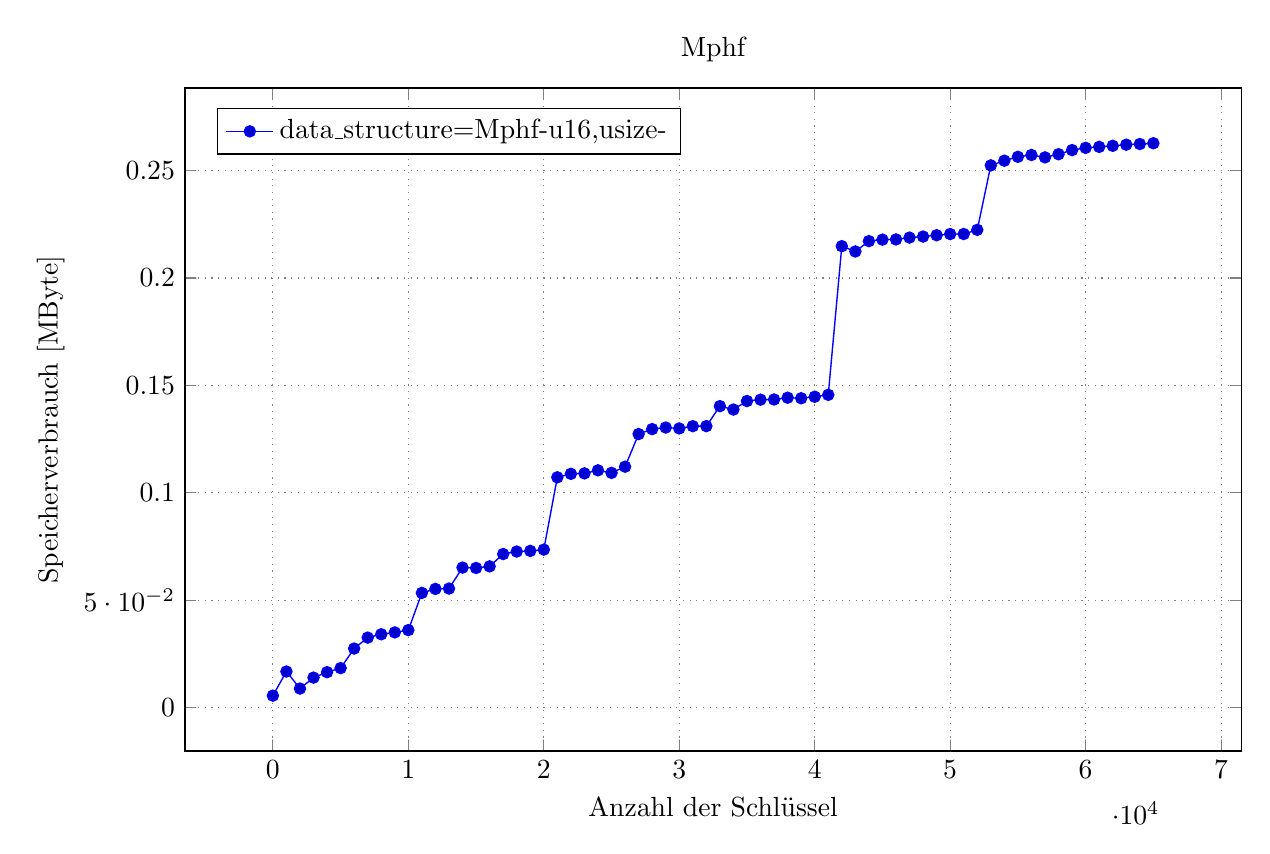
\begin{tikzpicture}
	\begin{axis}[
	title={Mphf},
	xlabel={Anzahl der Schlüssel},
	ylabel={Speicherverbrauch [MByte]},
	]
	
	%% MULTIPLOT(data_structure) SELECT size AS x, size_bytes/1e6 AS y, MULTIPLOT
	%% FROM mphf GROUP BY MULTIPLOT,x ORDER BY MULTIPLOT,x
 \addplot coordinates { (1,0.005626) (1001,0.016859) (2001,0.00892) (3001,0.01401) (4001,0.016548) (5001,0.018446) (6001,0.027546) (7001,0.032638) (8001,0.034188) (9001,0.035054) (10001,0.036132) (11001,0.053438) (12001,0.0553) (13001,0.055472) (14001,0.065224) (15001,0.065048) (16001,0.065798) (17001,0.071526) (18001,0.072696) (19001,0.073) (20001,0.073604) (21001,0.107256) (22001,0.108864) (23001,0.10908) (24001,0.110502) (25001,0.109304) (26001,0.11219) (27001,0.127384) (28001,0.129694) (29001,0.130416) (30001,0.129992) (31001,0.131056) (32001,0.131066) (33001,0.140376) (34001,0.13879) (35001,0.142746) (36001,0.143394) (37001,0.143472) (38001,0.144296) (39001,0.14405) (40001,0.144756) (41001,0.145636) (42001,0.214832) (43001,0.212368) (44001,0.217188) (45001,0.217872) (46001,0.217972) (47001,0.218842) (48001,0.219316) (49001,0.219924) (50001,0.220472) (51001,0.220488) (52001,0.22244) (53001,0.252438) (54001,0.254626) (55001,0.256426) (56001,0.257276) (57001,0.25616) (58001,0.25763) (59001,0.25955) (60001,0.260606) (61001,0.261052) (62001,0.26155) (63001,0.262068) (64001,0.262382) (65001,0.26274) };
 \addlegendentry{data\_structure=Mphf-u16,usize-};
 
	
	\end{axis}
	\end{tikzpicture}
\end{center}


\end{document}

%%%%%%%%%%%%%%%%%%%%%%%%%%%%%%%%%%%%%%%%%%%%%%%%%%%%%%%%%%%%%%%%%%%%%%%%%%%%%%%%
